% SC4051 --- Chapter 8: Case Studies (0->100)
\chapter{Case Studies: GFS, MapReduce, Kubernetes and Current Research}
\label{ch:case-studies}

\begin{quote}
\emph{``You cannot understand a system until you see how it behaves at scale, under failure, and under pressure.''} We close by tying every earlier chapter to real systems.
\end{quote}

\noindent\fbox{\parbox{\dimexpr\linewidth-2\fboxsep-2\fboxrule}{%
\textbf{From zero: from primitives to platforms.} We revisit foundations through four real systems---GFS, MapReduce, Kubernetes---and end with current research directions. Each case study maps to the models, clocks, RPC, consensus, replication, storage and transactions we have built.}}
\vspace{0.4em}

\section*{Learning Outcomes}
After this chapter you will be able to:
\begin{enumerate}[label=(L\arabic*)]
    \item explain GFS architecture and its consistency/availability trade-offs;
    \item describe MapReduce execution, fault tolerance and why it is not a general computation model;
    \item outline Kubernetes control-plane (etcd/Raft, controllers, scheduler) and reconciliation;
    \item map each case study to the earlier chapters (CAP, clocks, consensus, replication);
    \item identify two current research frontiers (serverless consistency, learned/distributed ML coordination).
\end{enumerate}

% ============================================================
\section{GFS: The Google File System}
\label{sec:gfs}
GFS (Ghemawat et al., 2003) was built for Google's workload: huge sequential reads/writes, append-heavy, thousands of clients, commodity disks that fail often. Design choices reflect those premises (and Ch.~1's fallacies taken seriously).

\paragraph{Architecture.} One \emph{master} (metadata: namespace, file $\to$ chunk mapping, chunk locations) and many \emph{chunkservers} (store 64\,MB chunks, $3\times$ replicated). Clients ask the master for chunk locations, then stream data directly to chunkservers---like HDFS but predating it. The master keeps all metadata in RAM for speed, with an operation log persisted and checkpointed.

\paragraph{Consistency model.} GFS offers \emph{relaxed} consistency: multiple writers appending to the same file may interleave, and the offset of an appended record is chosen by the primary chunkserver. Successful mutation is visible atomically at least once (at-least-once append), but failed retried appends can leave duplicates/padding that readers must handle. This is weaker than POSIX but sufficient for MapReduce-style batch pipelines where readers scan and filter.

\begin{figure}[h]
\centering
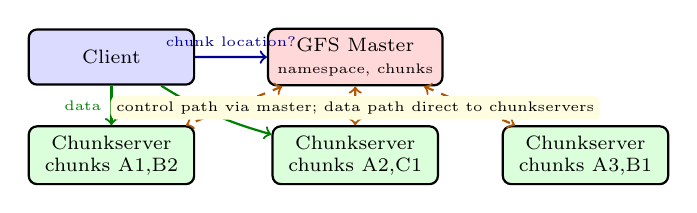
\begin{tikzpicture}[scale=0.86, every node/.style={font=\scriptsize},
  box/.style={draw,rounded corners=3pt,minimum width=2.1cm,minimum height=0.70cm,align=center,thick}]
\node[box,fill=red!15] (master) at (3.6,2.5) {GFS Master\\{\tiny namespace, chunks}};
\node[box,fill=blue!14] (client) at (0,2.5) {Client};
\node[box,fill=green!14] (cs1) at (0,1.05) {Chunkserver\\chunks A1,B2};
\node[box,fill=green!14] (cs2) at (3.6,1.05) {Chunkserver\\chunks A2,C1};
\node[box,fill=green!14] (cs3) at (7.0,1.05) {Chunkserver\\chunks A3,B1};
\draw[->,thick,blue!60!black] (client) -- (master) node[midway,above,font=\tiny] {chunk location?};
\draw[->,thick,green!50!black] (client) -- (cs1) node[midway,left,font=\tiny] {data};
\draw[->,thick,green!50!black] (client) to[bend right=8] (cs2);
\draw[<->,thick,orange!70!black,dashed] (master) -- (cs1) node[midway,left,font=\tiny] {heartbeat};
\draw[<->,thick,orange!70!black,dashed] (master) -- (cs2);
\draw[<->,thick,orange!70!black,dashed] (master) -- (cs3);
\node[font=\tiny,fill=yellow!12,rounded corners=2pt,inner sep=2pt] at (3.6,1.75) {control path via master; data path direct to chunkservers};
\end{tikzpicture}
\caption{GFS: single master for metadata, many chunkservers for data. Data bypasses the master after location lookup.}
\label{fig:gfs}
\end{figure}

GFS's single-master weakness (memory, availability) was addressed by Colossus (GFS2) with distributed metadata (Bigtable), and by HDFS Federation. The lesson: metadata scaling (Ch.~6) is often the first bottleneck to hit.

% ============================================================
\section{MapReduce: Data-Parallel Execution}
\label{sec:mapreduce}
MapReduce (Dean--Ghemawat, 2004) is a programming model plus a fault-tolerant runtime for batch processing over GFS-like storage.

\paragraph{Model.} Program two functions: \texttt{map}$(k_1,v_1)\to[(k_2,v_2)]$ and \texttt{reduce}$(k_2,[v_2])\to[(k_3,v_3)]$. The runtime shards input, runs $M$ map tasks, shuffles intermediate keys to $R$ reducers (grouping by $k_2$), and writes output back to GFS. The model is deliberately restricted: no iteration, no shared mutable state, no communication between mappers.

\paragraph{Fault tolerance.} Map tasks write intermediate output to local disk; on failure the task is re-executed elsewhere (deterministic replay). Reduce tasks read shuffled data; failed reducers re-read from map outputs. The master (coordinator) tracks liveness via heartbeats and reschedules. Stragglers are mitigated by \emph{backup tasks} (speculative execution): run a duplicate of the slowest tasks and take the first result---a direct application of tail-latency handling.

\begin{figure}[h]
\centering
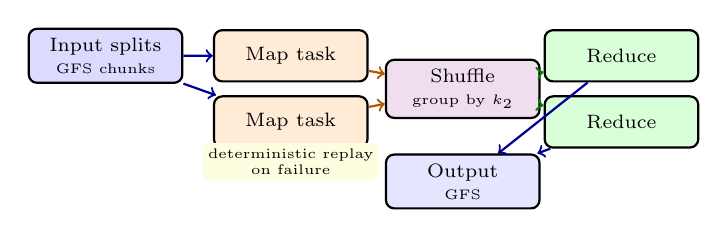
\begin{tikzpicture}[scale=0.84, every node/.style={font=\scriptsize},
  box/.style={draw,rounded corners=3pt,minimum width=1.95cm,minimum height=0.65cm,align=center,thick}]
\node[box,fill=blue!14] (input) at (0,2.2) {Input splits\\{\tiny GFS chunks}};
\node[box,fill=orange!16] (map1) at (2.8,2.2) {Map task};
\node[box,fill=orange!16] (map2) at (2.8,1.2) {Map task};
\node[box,fill=violet!13] (shuf) at (5.4,1.7) {Shuffle\\{\tiny group by $k_2$}};
\node[box,fill=green!15] (red1) at (7.8,2.2) {Reduce};
\node[box,fill=green!15] (red2) at (7.8,1.2) {Reduce};
\node[box,fill=blue!10] (out) at (5.4,0.30) {Output\\{\tiny GFS}};
\draw[->,thick,blue!60!black] (input) -- (map1);
\draw[->,thick,blue!60!black] (input) -- (map2);
\draw[->,thick,orange!70!black] (map1) -- (shuf);
\draw[->,thick,orange!70!black] (map2) -- (shuf);
\draw[->,thick,green!50!black] (shuf) -- (red1);
\draw[->,thick,green!50!black] (shuf) -- (red2);
\draw[->,thick,blue!60!black] (red1) -- (out);
\draw[->,thick,blue!60!black] (red2) -- (out);
\node[font=\tiny,align=center,fill=yellow!12,rounded corners=2pt,inner sep=2pt] at (2.8,0.60) {deterministic replay\\on failure};
\end{tikzpicture}
\caption{MapReduce dataflow: input $\to$ map $\to$ shuffle (group) $\to$ reduce $\to$ output. Failures are handled by re-execution; stragglers by backup tasks.}
\label{fig:mapreduce}
\end{figure}

\begin{lstlisting}[language=Python]
# MapReduce word count -- the canonical example (runnable locally)
from collections import defaultdict

def map_fn(doc_id, text):
    for word in text.lower().split():
        yield (word, 1)

def reduce_fn(word, counts):
    yield (word, sum(counts))

# Simulate execution with fault tolerance via re-execution
docs = [(1,"hello world hello"), (2,"world of distributed systems"),
        (3,"hello distributed world")]

# Map phase: each doc is a split; map is deterministic so replay is safe
intermediate = defaultdict(list)
for doc_id, text in docs:
    for k, v in map_fn(doc_id, text):
        intermediate[k].append(v)

# Shuffle is implicit in the dict grouping above
# Reduce phase
output = {}
for word, counts in intermediate.items():
    for k, v in reduce_fn(word, counts):
        output[k] = v

print(sorted(output.items()))
# [('distributed', 2), ('hello', 3), ('of', 1), ('systems', 1), ('world', 3)]

# Straggler mitigation: backup task (first result wins) -- sketch
import concurrent.futures
def slow_map(doc):  # one task is slow
    import time; time.sleep(0.05 if doc[0]==2 else 0)
    return list(map_fn(*doc))

with concurrent.futures.ThreadPoolExecutor() as ex:
    futs = {ex.submit(slow_map, d): d for d in docs}
    for fut in concurrent.futures.as_completed(futs):
        pass  # in real MR, duplicate slowest and take first
\end{lstlisting}

MapReduce's limitation---no efficient iteration---led to Spark (in-memory RDDs), Flink (streaming) and Dataflow. The core insight remains: restrict the model to make fault tolerance and scheduling tractable.

% ============================================================
\section{Kubernetes: Reconciliation and the Control Plane}
\label{sec:k8s}
Kubernetes orchestrates containers at scale. Its architecture maps directly to earlier chapters: etcd (Raft, Ch.~4) for consistent state, controllers that reconcile desired vs.\ actual state (a replication idea, Ch.~5), and a scheduler that places pods.

\paragraph{etcd (Raft).} All cluster state (pods, services, config) lives in etcd, a Raft-replicated key-value store (Ch.~4). Every write is linearizable; the AP side is handled by kubelet caching on each node so workloads survive etcd unavailability briefly.

\paragraph{Reconciliation loop.} Controllers watch etcd, compare desired state (the spec in etcd) with actual state (what kubelets report), and act to converge them---a continuous control loop, not a one-shot RPC. This makes the system self-healing under Ch.~1's fallacies: messages lost, nodes crash, controllers simply re-reconcile.

\begin{figure}[h]
\centering
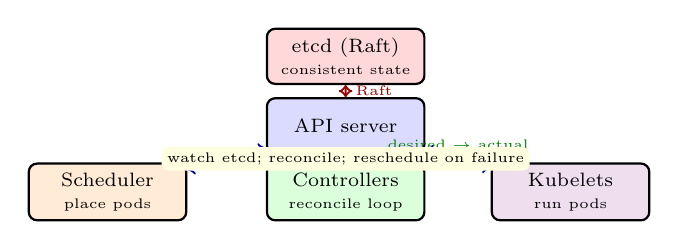
\begin{tikzpicture}[scale=0.84, every node/.style={font=\scriptsize},
  box/.style={draw,rounded corners=3pt,minimum width=2.0cm,minimum height=0.70cm,align=center,thick}]
\node[box,fill=red!15] (etcd) at (3.6,2.6) {etcd (Raft)\\{\tiny consistent state}};
\node[box,fill=blue!14] (api) at (3.6,1.55) {API server};
\node[box,fill=orange!16] (sched) at (0,0.55) {Scheduler\\{\tiny place pods}};
\node[box,fill=green!14] (ctrl) at (3.6,0.55) {Controllers\\{\tiny reconcile loop}};
\node[box,fill=violet!13] (kubelet) at (7.0,0.55) {Kubelets\\{\tiny run pods}};
\draw[<->,thick,red!60!black] (etcd) -- (api) node[midway,right,font=\tiny] {Raft};
\draw[<->,thick,blue!60!black] (api) -- (sched);
\draw[<->,thick,blue!60!black] (api) -- (ctrl);
\draw[<->,thick,blue!60!black] (api) -- (kubelet);
\draw[->,thick,green!50!black,dashed] (ctrl) to[bend left=18] node[midway,above,font=\tiny] {desired $\to$ actual} (kubelet);
\node[font=\tiny,fill=yellow!12,rounded corners=2pt,inner sep=2pt] at (3.6,1.05) {watch etcd; reconcile; reschedule on failure};
\end{tikzpicture}
\caption{Kubernetes control plane: etcd (Raft) stores desired state; controllers and scheduler reconcile actual state toward it.}
\label{fig:k8s}
\end{figure}

\begin{lstlisting}[language=Python]
# Reconciliation loop: desired vs actual state (Kubernetes controller pattern)
import time

desired = {"replicas": 3}   # spec in etcd
actual = {"pods": []}       # reported by kubelets

def reconcile(desired, actual):
    need = desired["replicas"] - len(actual["pods"])
    if need > 0:
        for i in range(need):
            pod = f"pod-{len(actual['pods'])+1}"
            actual["pods"].append(pod)
            print(f"  created {pod}")
    elif need < 0:
        for _ in range(-need):
            pod = actual["pods"].pop()
            print(f"  deleted {pod}")
    return actual

# Simulate: start, scale up, node failure, scale down
for step in ["init", "node failure (lose 1 pod)", "scale to 5", "scale to 2"]:
    print(f"\n[{step}] desired={desired} actual={actual}")
    if step == "node failure (lose 1 pod)":
        actual["pods"].pop()
    if step == "scale to 5": desired["replicas"] = 5
    if step == "scale to 2": desired["replicas"] = 2
    reconcile(desired, actual)
    print(f"  -> actual={actual}")
\end{lstlisting}

% ============================================================
\section{Current Research Frontiers}
\label{sec:research}
Two directions tie the course together:

\paragraph{Serverless and strong consistency.} Serverless functions are stateless and short-lived; coordinating them with strong guarantees (exactly-once workflows, distributed transactions across functions) is an active area (Beldi, Olive, Cloudburst). The tension is Ch.~2--4 at the extreme: no stable process to hold a lock, yet the application wants transactions.

\paragraph{ML coordination at scale.} Training large models needs parameter synchronisation across thousands of GPUs. Choices mirror Ch.~5: synchronous all-reduce (BSP, strong consistency, straggler-sensitive) vs.\ asynchronous parameter servers (stale gradients, faster but noisy) vs.\ bounded-staleness (SSP). Emerging work uses in-network aggregation and RDMA to push replication into the fabric itself.

Both frontiers ask the same question the course began with: what guarantees can we provide when the network is unreliable, clocks diverge and machines fail independently? The primitives---quorums, vector clocks, consensus, commit protocols---reappear, just at new scales and with new hardware.

% ============================================================
\section{Exercises}
\label{sec:ch08-exercises}
\begin{enumerate}[label=E8.\arabic*, leftmargin=*, itemsep=0.6em]
    \item \textbf{GFS consistency.} Two clients concurrently append to the same GFS file. Explain why the file may contain interleaved records and duplicates after retries. How does MapReduce tolerate this when reading GFS output? Propose a record format that makes duplicates detectable.
    \item \textbf{MapReduce stragglers.} A job has 1000 map tasks; 5 are 10$\times$ slower (stragglers). Without backup tasks the job takes $T$. With backup tasks that duplicate the slowest 10 tasks after 80\% completion, estimate the speedup. When does speculation hurt (cost vs.\ benefit)?
    \item \textbf{Kubernetes and Raft.} etcd uses Raft with 5 members. How many failures can it tolerate for reads and writes? If etcd is partitioned 3--2, which side serves linearizable writes? How do kubelets keep pods running during the partition?
    \item \textbf{Putting it together.} Map each case study (GFS, MapReduce, Kubernetes) to chapters 1--7: identify the failure model, timing assumption, consistency level, replication strategy and coordination mechanism it uses. Present as a table.
    \item \textbf{Research design.} Design a serverless workflow that must atomically update two Dynamo-style stores (eventual). Propose a solution using idempotency keys plus a transaction coordinator (2PC-like). Analyse what happens if the coordinator crashes mid-workflow and how you would make it highly available.
\end{enumerate}

% ============================================================
\section*{Chapter Notes}
GFS: Ghemawat--Gobioff--Leung (SOSP, 2003); Colossus/Bigtable evolution in Corbett et al.\ (2012). MapReduce: Dean--Ghemawat (OSDI, 2004); Spark: Zaharia et al.\ (NSDI, 2012); Dataflow: Akidau et al.\ (VLDB, 2015). Kubernetes: Burns et al., \emph{Borg, Omega, and Kubernetes} (CACM, 2016); etcd/Raft documentation. Serverless consistency: Zhang et al., ``Cloudburst'' (VLDB, 2020); Beldi (OSDI, 2020). ML coordination: Li et al., ``Scaling distributed ML with parameter server'' (OSDI, 2014); SSP: Ho et al.\ (2013).

% End of Chapter 8
